\section{Evaluation of real-time interactions between the user and the agent}
\label{sec:eval}

%We present in this section an evaluation of an embodied conversational agent coordinating turns in real time with users in the context of a negociation scenario.

\subsection{Motivation}
\label{subsec:mot}

This evaluation aimed at answering three questions: 
%\begin{enumerate}
%\item
(i) Is an agent controlled by our model able to coordinate smoothly its speaking turns with the user?
%\item
(ii) How the user perceives the agent's interruptions as controlled by our model?
%\item
(iii) How different turn-taking behaviors impact agent's credibility, user's satisfaction and easiness to interact with the agent? Do different turn-taking behaviors influence the user's turn-taking behavior? 
%\end{enumerate}

%To that purpose we chose to inspire from 
Our methodology was based on existing evaluations techniques.
\cite{skantze_towards_2010} and \cite{de_vault_toward_2015} conducted two studies to evaluate agent's turn-taking in the context of negociation scenarios. In these two experiments, the agents were at least partially controlled by a Wizard of Oz (WOz). In \cite{skantze_towards_2010} only the user's utterances were transcribed by the WOz, the remaining being managed by the system. User's ends of turn were identified using a voice activity detector and the system systematically responded to the user after detecting the end of the user's turn. In \cite{de_vault_toward_2015}, the whole process, from interpretation to generation, was managed by the Wizard of Oz, including turn-taking management. These two experiments had the advantage to answer research questions similar to ours. First, the agent's coordination ability was evaluated by comparison of the agent's response time and overlap duration with human interactions. Second, the agent's credibility, the user's satisfaction and easiness to interact with the agent were evaluated through questionnaires. The ability of the agent to correctly signal its intentions towards turn-taking was not directly treated. However some behaviors of the user were analyzed in these evaluations such as the user latency to take the turn after the end of the agent's turn. To our view, these behaviors could be related to the ability of the user to clearly identify signals displayed by the agent, the clearer the agent's signals, the shorter the user's response latencies. These evaluations seemed particularly adapted to our own objective and thus we based our methodology on them. Nevertheless, one major difference is that, in our case, the agent's turn-taking behaviors varied according to the outputs of our model. 

\subsection{Protocol}

Similarly to \cite{de_vault_toward_2015} and \citep{skantze_towards_2010}, we conducted an experiment where the user was engaged in a negociation scenario with the agent. The interaction was only audio, the agent had no graphical representation and only perceived and controlled two prosodic parameters, the loudness and the pitch. 
%In the negociation scenario, both participants are on a sinking boat, and prepare to 
The scenario staged two participants on board a sinking boat, preparing to embark on a life boat. 
Each participant had different beliefs on the situation. 
One thought that they wre close to the coast, in this situation the priority was thus to reach the coast as soon as possible. 
The other thought they were far from the coast, the priority being here to survive as long as possible. 
Given their different beliefs, they had to make a share decision about three items to take away in the life boat among six. We choose the different items such as three of them were adapted to first situation 
%where participants are close to the coast 
and three to the second one.
%objects were adapted to situations were participants are far from the coast. 
The scenario conducted the user, given his own belief, to disagree with the agent's proposals.   
% Déplacé en second paragraphe

We used our implementation presented in section \ref{impl}. The agent had thus a complete turn-taking module that determined when the agent utterance should be launched. In order to avoid user's utterances misinterpretations we chose to replace the Automatic Speech Recognizer and Response Planning components by a Wizard of Oz. The WOz listened and selected utterances thanks to an interface that allowed to select arguments in favor of the items the agent wanted to take and to produce counter-arguments to the user's proposals. It was necessary to avoid any influence of the Wizard of Oz response time on the agent turn-taking behavior. To that purpose, the WOz was instructed to select the agent's next utterance before the end of the user's utterance. 
To make the WOz answering as fast as possible, the interface was organised in buttons, determining the different dialog acts. Once the Wizard of Oz selected a particular dialog act by clicking the corresponding button, an utterance related to this dialog act was chosen among a list of utterances, allowing the agent to vary its answers to the user. The utterance chosen was then sent to the agent that determined when to launch the utterance according to the output of the turn-taking module, using the mechanism presented in section \ref{impl}. In order to have the most natural interactions, the different utterances that the agent could produced were collected from a corpus of human interactions we collected before. 

% Déplacé en troisième paragraphe
In order to assess the ability of our agent to coordinate with the user, we compared our turn-taking model (M1) with an implementation of a second model (M2). 
In this second model, we used a voice activity detector to discriminate moments when the user spoke from moment of silence. 
%Given the result of the voice activity detector,
The second turn-taking module was implemented following the following rules: 
\begin{itemize}
\item when no speech activity is detected after 600~ms, consider that the user has finished its turn and take the turn;
\item after at least 100~ms of speech activity, consider that the user is beginning a new turn and stop speaking. 
\end{itemize} 
These rules based on temporal threshold are often used in spoken dialog systems and agent architectures \citep{ward_root_2005}. Interestingly, they are considered as non-optimal \citep{ward_root_2005}. The two thresholds of 600~ms and 100~ms corresponded to values used in existing models (see for example \citep{ferrer_is_2002}). 

When the agent was controlled by our model M1, it was able to modulate its prosodic signals and thus to inform the user about its intentions by decreasing the pitch and loudness of its voice at the end of the turn and raising its pitch and loudness to inform the user about its intention to grab the turn.  
With model M2, the agent was not able to vary its prosodic signals and thus had no nonverbal modality to convey any information about its intentions. 

In order to assess whether the agent turn-taking behavior influenced the user's judgement and behavior, we defined two different behaviors according to the agent's role. In the first case, the agent systematically released the turn when it detected that the user wanted to grab the turn, and systematically waited the end of the user's turn before taking the turn (weak motivation to take or to keep the turn). In the second case, the agent insisted to keep the turn when it detected that the user wanted to grab the turn, and systematically tried to grab the turn (strong motivation to take or to keep the turn). In order to generate the two behaviors, we varied the motivation value. 
For the first behavior, $m=-0.4$ when the agent was the speaker and $m=0.4$ when the agent was the listener. In the second condition, $m=-1.0$ when the agent was the speaker, and $m=1.0$ when the agent was the listener.

We ensured that the user interacted equally with the agent having respectively weak and strong motivation to take or keep the turn. To that purpose, we divided the interaction in two parts. In the first part the user interacted with an agent having a weak motivation to take or keep the turn, and in the second part with an agent with a strong motivation.
% the user interacted with an agent having a strong motivation to take and keep the turn. 
We kept this order for all the interactions, because beginning the interaction with an agent systematically trying to grab or to keep the turn would risk to make the user to refuse to continue to engage in the interaction with the agent. 

Finally, the user's judgements about the agent were collected using a questionnaire presented in table \ref{Answers}, which included questions about the easiness to interact with the agent (question Q9 in table \ref{Answers}), user's satisfaction (Q8, Q10) and agent credibility (Q11). The corresponding questions were adapted from \cite{skantze_towards_2010}, \cite{bevacqua_effects_2014} and \cite{de_vault_toward_2015}. Moreover, in order to assess the clarity of the agent's signals, we added questions about the intentionality of agent's interruptions, that is whether interruptions of the agent were due to an agent mistakenly perceiving the user's ends of turn or where made by the agent on purpose (Q3, Q4). Finally, we added questions about the ability of the agent to smoothly coordinate its turns with the user (Q1, Q2, Q5, Q6, Q7). For each items, the participant had to declare its level of agreement, between strongly disagree and strongly agree in a continuous scale between 0 and 10. 
%The different items were inspired from \cite{skantze_towards_2010}, \cite{bevacqua_effects_2014} and \cite{de_vault_toward_2015}.

%As a result, we had two main conditions,
The different conditions of the experiment were as follows.
In condition 1 the user interacted with an agent controlled by model M1.
In condition 2, the user interacted with an agent controlled by model M2.
Condition 1 presented to variants, depending of the value of the motivation parameter: ``condition 1 strong'' and ``condition 1 weak''. 
% We chose to name the first part of the condition 1, when the user interacted with an agent having a weak motivation to keep and take the turn ``condition 1 weak", and the second part of the ``condition 1 strong", when the user interacted with an agent having a weak motivation to keep and take the turn ``condition 1 strong". 
Each participant interacted twice with the agent, each time with a different condition.
The order of the conditions (``condition 1" and ``condition 2") was counterbalanced between participants. For each condition, the interaction lasted 2 min 30 s. The questionnaire was presented to the participant at the end of each condition.


\section{Results}

31 volonteers (30 men and 1 woman) participated to the experiment. They were all native French speakers and were students, engineers or researchers. We describe in the following sections the analysis we made to answer the three questions presented section \ref{subsec:mot}.

\subsection{Is the agent able to coordinate smoothly with the user?}

First, we analyzed the duration of the user to agent transitions (Figure \ref{box_ua}). It assessed the ability of the agent to rapidly identify and react to the user's end of turn. For this analysis, we annotated manually the turns of the participants. Then, we kept only transitions that were not overlaps nor transitions that were not anticipated by the agent. We found that in ``condition 1 weak", the agent took the turn more rapidly (average: 840~ms) compared to the second condition (1.19~s), the difference being significant (p$<$0.05). However, we also observed a high number of mistakes in the detection of user's ends of turn, whatever the condition, with almost 50 \% of transitions having at least slight overlaps.  
Finally, we analyzed the responses to questions Q1, Q2, Q5, Q6 and Q7 (table \ref{Answers}), referring to the user's subjective perception of the agent's ability to coordinate its speaking turns. We did not found significant differences between both conditions. Generally speaking, participants found that the agent was able to coordinate its turn with the user, with low scores for questions Q1, Q2 and Q6. They logically found that the agent paid more attention not to interrupt them in condition 2 compared to condition 1 (question Q5). Nevertheless, the answers to question Q7 showed that users noticed long moments of silence where the agent did not seem to want to speak. 
 
\begin{figure}
\centering
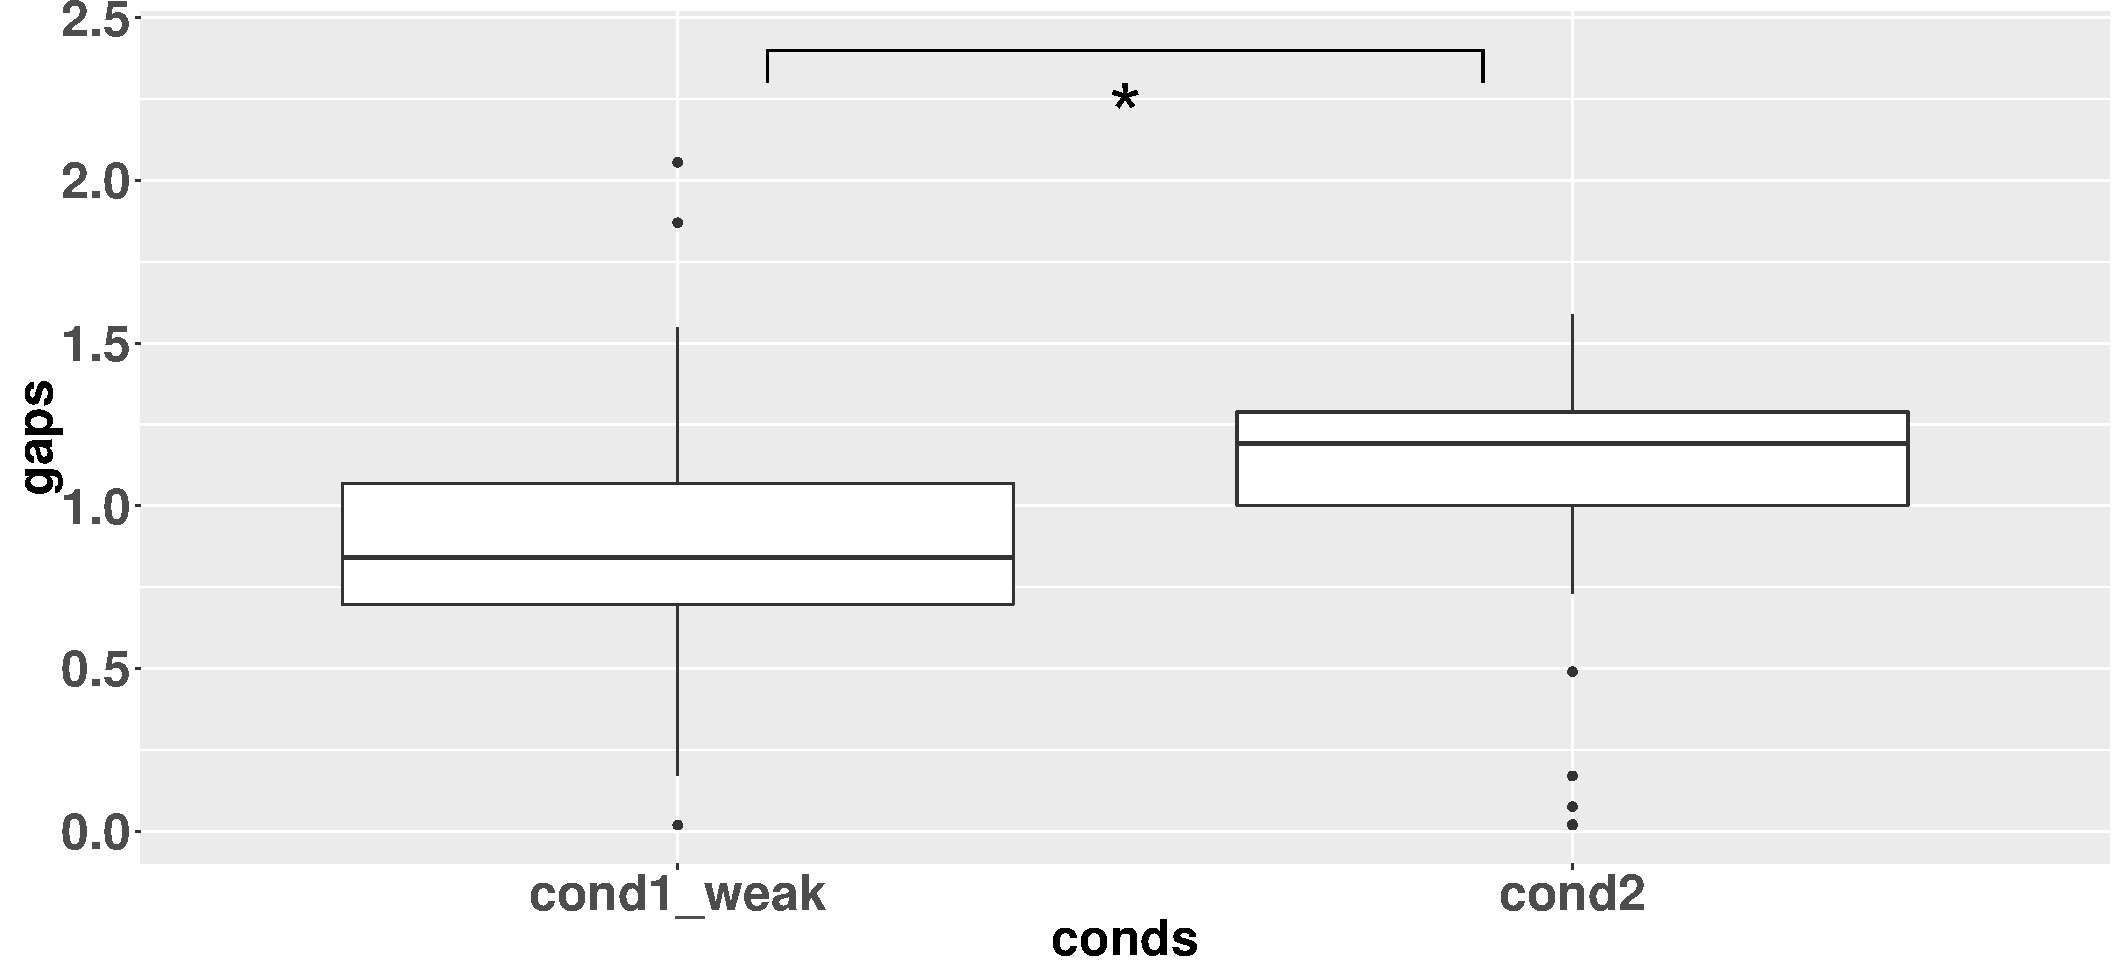
\includegraphics[width=\linewidth]{figure/boxTransitionsUA.pdf}
\caption{Durations of silence during User to Agent transitions (gaps in seconds).}
\label{box_ua}
\end{figure}
  
\begin{table}
\centering
\resizebox{\linewidth}{!}{\begin{tabular}{|p{3cm}|p{2cm}|p{2cm}|p{2cm}|}
\hline
Questions & Median \linebreak conds. 1 & Median \linebreak cond. 2 & p-value \\
\hline
Q1: My interlocutor \linebreak didn't perceive the moment were I talked & 2.25 & 1.75 & 0.95\\
\hline
Q2: My interlocutor took the turn randomly& 2.5 & 2.625 & 0.6 \\
\hline
Q3: My interlocutor interrupted involuntarily& 6 & 4 & 0.019* \\
\hline
Q4: My interlocutor interrupted me on purpose& 6 & 6.5 & 0.91 \\
\hline
Q5: My interlocutor paid attention not to interrupt me & 4.5 & 7.5 & 0.006**\\
\hline
Q6: My interlocutor was slow to respond to me & 3 & 2 & 0.77\\
\hline
Q7: My interlocutor refused sometimes to speak to me & 6.125 & 5.75 & 0.16\\
\hline
Q8: My interlocutor annoyed me by the way he took the turn & 4.5 & 3.25 & 0.54\\
\hline
Q9: I was at ease interacting with my interlocutor & 5.25 & 6.25 & 0.55\\
\hline
Q10: I liked speaking with my interlocutor & 6.625 & 7 & 0.52\\
\hline
Q11: The behavior of my interlocutor was close to the behavior of a human speaker & 5.625 & 6.5 & 0.97\\
\hline
\end{tabular}}
\caption{Mean agreements of the participants for conditions 1 and condition 2 (translated from French).}
\label{Answers}
\end{table}

\subsection{How the user perceives the agent's interruptions?}

By analyzing the answers to questions Q3 and Q4, we found that users classified the agent's interruptions as intentional or unintentional in condition 1 (scores higher than 5 for the two conditions) even if users only slightly agreed with assertions Q3 and Q4. Logically, participants perceived that the agent paid more attention not to interrupt them in condition 1, compared to condition 2. 
We completed this analysis with measures of the user's behavior during interruptions. We found that the pitch of the user was significantly greater than the mean pitch during conflictual moments, for ``condition 1 strong''. It means that in this condition, the user seemed to react in a specific manner to the interruptions made on purpose by the agent. Such reaction was not be observed in the other conditions where the agent overlapped involuntarily the user's speech.


\begin{figure}
\centering
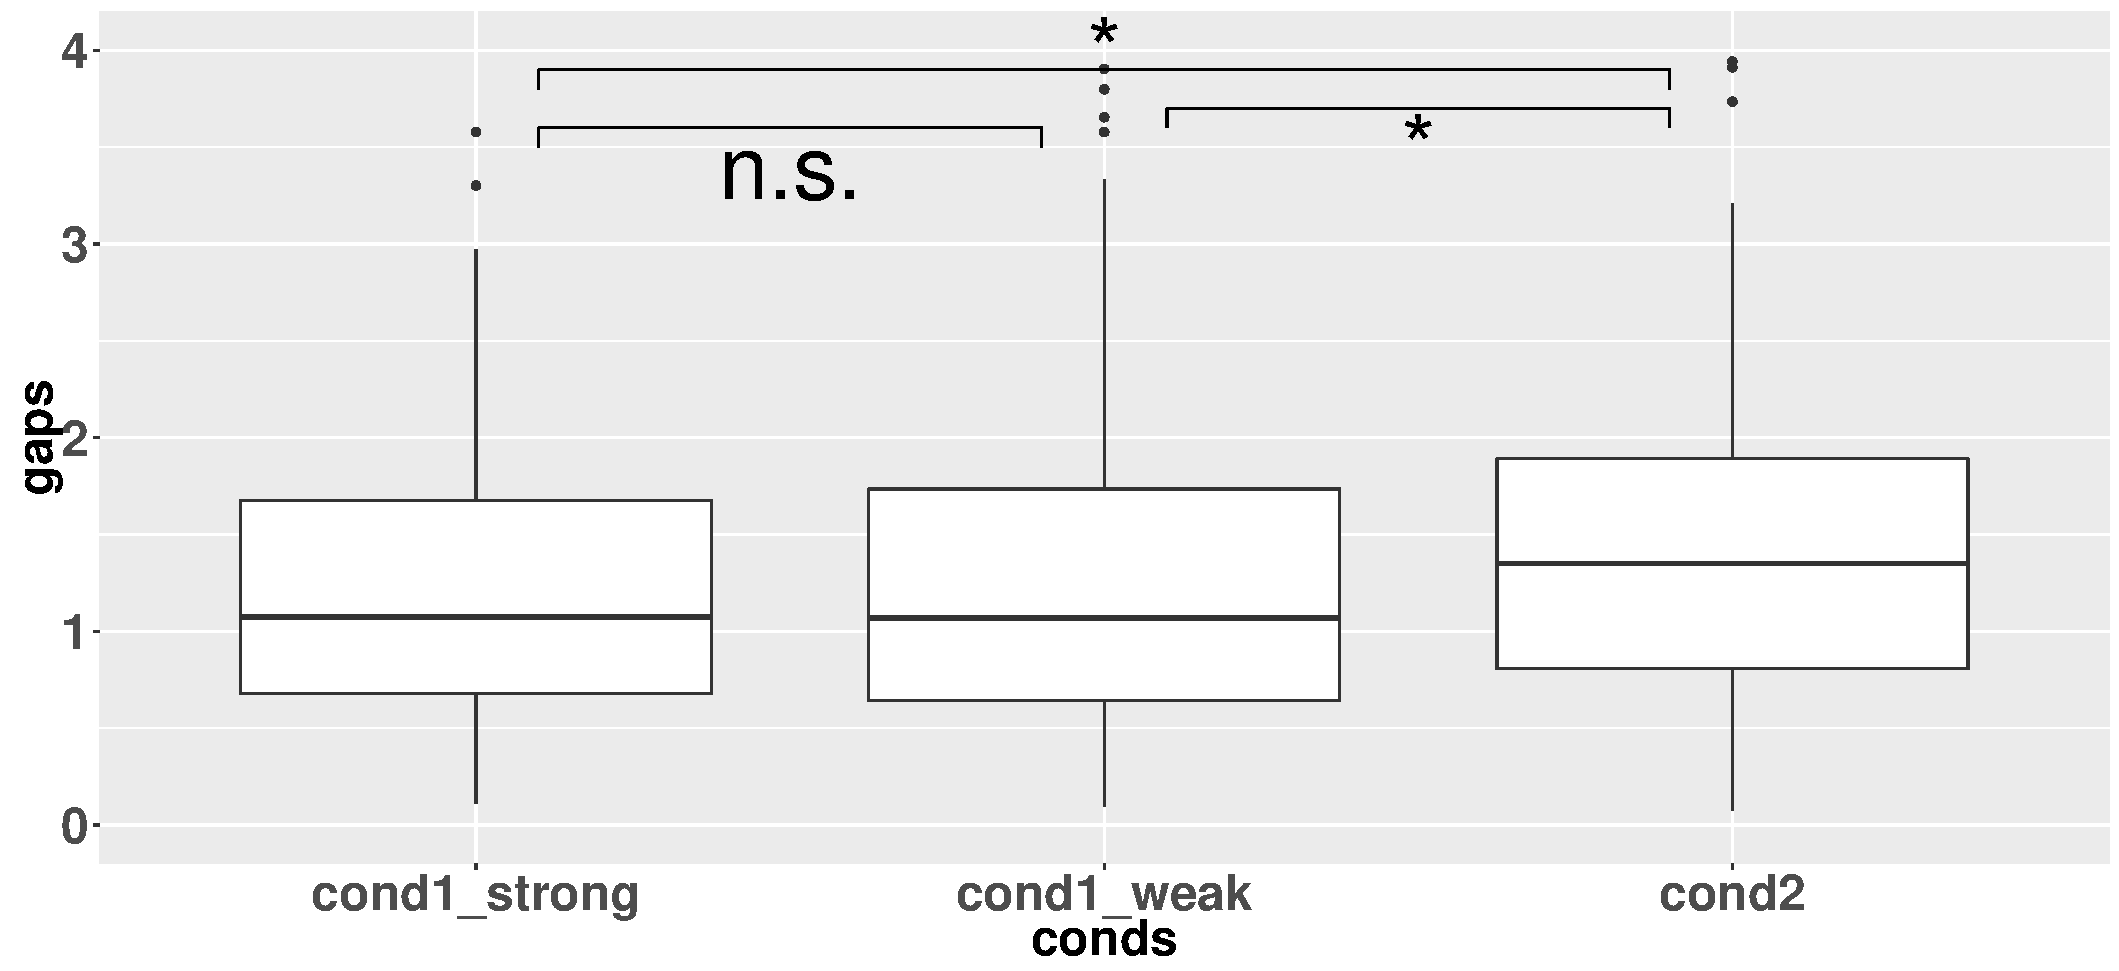
\includegraphics[width=\linewidth]{figure/boxTransitionsAU.pdf}
\caption{Durations of silence during Agent to User transitions (gaps in seconds).}
\label{box_au}
\end{figure}

\subsection{How different turn-taking behaviors impact agent's credibility,  user's satisfaction and easiness to interact with the agent?}

Generally speaking, participants liked speaking with the agent (question Q10). The results to the question related to the credibility of the agent were more mitigated (Q11), with a median value of 6.5 to the assertion "The behavior of my interlocutor was close to the behavior of a human speaker" in the second condition and of 5.625 for the first condition. Users also answered that they were at ease in the interaction (Q9), even if they did not strongly agree with the assertion, and seemed not annoyed by the agent's turn-taking behavior (Q8). 
We finally, assessed the impact of the condition on the user's ability to coordinate himself with the agent by measuring the duration of agent to user transitions. We found that in the condition 1, the user took the turn more rapidly (average: 1.11~s) compared to condition 2 (average: 1.39~s), the difference being significant (p$<$0.05). 


\subsection{Discussion}

Results show that our model allows the agent to smoothly coordinate its turns with users. Indeed, while unintentional overlaps, due to mistakes in the perception of the user end of turn, do not seem to differ between conditions, the agent took the turn faster in ``condition 1 weak", compared to ``condition 2". The high rate of false detections of the end of turn by the two models (50 \% of user-agent transitions) can be partially due to the voice activity detector used to detect when the user was speaking: logs revealed a great number of moments where no voice was detected whereas the user was actually speaking. 
Answers to questions Q1, Q2, Q6 and Q7 show that users did not clearly perceive the improved coordination capability brought by our model. The fact that the participants did not seem to be disturbed by the relatively long duration of user to agent transitions supports the idea that they did not expect optimal turn transitions from the agent.

Moreover, when investigating how users perceived the agent's interruptions, we observed that users considered almost equally that the agent interrupted them unintentionally or on purpose, as well when the agent raised its volume and pitch to inform the user about its intention to grab the turn (our model), and when the pitch and volume were not modulated. However, we found that users increased their pitch when interrupted by the agent only in ``condition 1 strong". This lead us to think that users distinguished, at least implicitly, the intentional or unintentional character of the interruptions and varied their behavior accordingly. We can conclude that solely raising pitch and loudness did not seem to sufficiently inform the agent's intention to grab the turn. The lack of distinction between intentional interruptions and those due to mistakes in the detection of the user end of turn could be due to difficulties of the participants to perceive the prosodic variations of the agent. These difficulties could come from the quality of the voice synthesizer we used, participants having often reported the poor quality of the voice. 
At the end of the experiment, we collected the oral impressions of the participants about the interaction. Participants were divided when asked about their perception of the agent's interruptions. Six participants explicitly mentioned that they perceived the interruptions of the agent as non-voluntary, on the opposite, thirteen participants perceived at least some interruptions as voluntary. 

 As a result, we found that users took the turn faster with our model. Two hypotheses can explain this difference. 
%First, users could have perceived the decrease in pitch and loudness made by the agent to inform its intention to release the turn, this perception helping the user to identify the agent's end of turn. 
First, users could have perceived the decrease in pitch and loudness in the agent's voice, helping them to identify the agent's willingness to end its turn. 
Second, differences in agent-user transition durations could be the result of an alignment effect: the fact that the agent took the turn faster led the user to take the turn faster. This hypothesis is plausible, as such alignment has been observed in human conversations \citep{levitan_entrainment_2015}.  

%Finally, the results show that varying the agent's behavior do not seem to impact user's judgement about the interaction, as answers to questions Q8, Q9, Q10 and Q11 are not significantly higher for condition 1 compared to condition 2. Moreover, answers to these questions do not strongly favorize positive impressions about the agent. However, oral impressions collected after the interaction are not so categorical.   
Finally, the analysis of the answers to the questionnaire shows that the variation the agent's behavior do not seem to impact user's judgement about the interaction. Nevertheless, results do not strongly favor positive impressions about the agent. However, oral impressions collected after the interaction are not so categorical.   
For example, perception of the interruption seems to conduct to more positive impressions. Four participants judged interruptions as coherent and credible given the dialog context, and five participants associated these interruptions to the fact that the agent did not agree or tried to impose its own ideas, which is consistent. 
Finally, among the thirteen participants, five of them judged these interruptions as human-like. On the opposite, one of the participants reported a feeling of rage linked to the incessant interruptions of the agent, and two participants reported that they were annoyed by these interruptions. We could explain the differences in the impressions given by interruptions by the fact that the agent interrupted the user regardless of the dialog context. This could result in moments where the agent's interruptions seemed not appropriate given the context of the dialog, while other interruptions were particularly relevant to the context. Interruptions could thus give an impression of smoothness and immersion in the dialogue to the condition that they are consistent with the context of the dialog, what the variation of the motivation parameter of our model is supposed to provide.
